\thispagestyle{fancy}
\begin{center}
	\LARGE{\textbf{Ley de ohm (Segunda parte)}}
\end{center}
\section{Objetivos}
Al finalizar esta experiencia, usted estará capacitado para:
\begin{enumerate}
	\item Demostrar la primera ley de Ohm en forma experimental.
	\item Determinar el valor de los resistores, a partir de los valores medidos de tensión y corriente.
	\item Determinar la corriente en un circuito a partir de la resistencia (determinada mediante el código de colores) y la tensión medida.
	\item Determinar la tensión en un circuito a partir de la resistencia (leída mediante el código de colores) y de la corriente medida con un amperímetro.
\end{enumerate}

\section{Conocimientos previos}
La ley de Ohm establece que la tensión en bornes de un resistor es igual al producto de su resistencia por la corriente que circula por el resistor.
Esta ley puede ser utilizada para cálculo de la tensión, corriente y la resistencia. 
Las ecuaciones son:
\begin{equation*}
	V=I*R 
\end{equation*}
\begin{equation*}
	I=V/R
\end{equation*}
\begin{equation*}
	R=V/I
\end{equation*}
Donde:
\begin{itemize}
	\item \textbf{V} tensión a través de resistor del resistor (en V)
	\item \textbf{I} corriente que circula por el resistor (en A) 
	\item \textbf{R} resistencia del resistor (en $\Omega $ )
\end{itemize}
\section{Equipo}
El siguiente equipo es necesario para realizar la experiencia.
\begin{enumerate}
	\item Modulo de experimentos
	\item Uno o dos DMM (Multímetros)
\end{enumerate} 
\section{Procedimiento}
\begin{enumerate}
	\item Estudie e implemente el circuito de la figura 1
	\\
	\\
	\begin{figure}[h]
		\begin{minipage}{0.4\textwidth}
			\centering
			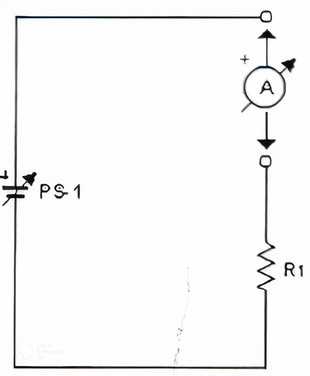
\includegraphics[width=\textwidth]{imagenes/4.1}
			\caption{Primera medición}
			\label{fig:imagen1}
		\end{minipage}%
		\begin{minipage}{0.5\textwidth}
			\centering
			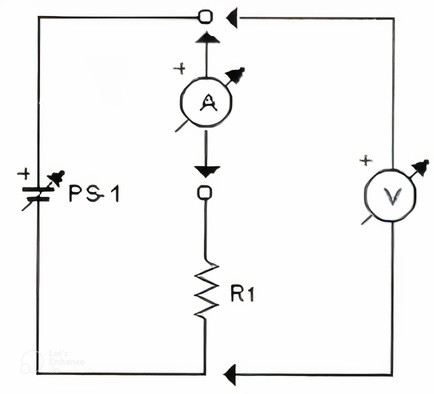
\includegraphics[width=\textwidth]{imagenes/4.2}
			\caption{Segunda medición}
			\label{fig:imagen2}
		\end{minipage}
	\end{figure}
	\item Estudie y efectué los cálculos teóricos para el circuito en la figura 1, utilizando los valores del cuadro 1. 
	\item Ajuste la tensión de la alimentación  PS-1 a 0 V.
	\item Ajuste el multímetro como amperímetro en la escala de 20 mA.
	\item Conecte el circuito como se muestra en la figura 2. Note que el multímetro está conectado para medir la corriente en $R_{1}$.
	\item Ajuste la fuente de alimentación para que la corriente sea 0 mA ( el primer valor en el  siguiente cuadro).
	\\ Las resistencias usadas son los siguientes:$R_{1}=4k\Omega$ y $R_{2}=2k\Omega$
	\begin{table}[htbp]
		\centering
		
		\begin{tabular}{|c|c|c|c|c|}
			\hline
			Corriente en $R_{1}$ y $R_{2}$&\multicolumn{2}{ |c}Tensión en $R_{1}$ (V)&\multicolumn{2}{ |c} Tensión en $R_{2}$ (V) \\
			\hline
			&Calculado&Medido&Calculado&Medido\\ \hline
			0 mA & 0 &  0 & 0& 0 \\ \hline
			0.2 mA & 0.8 &  0.81 & 0.4& 0.42 \\ \hline
			0.4 mA & 1.6 &  1.6 & 0.8& 0.75 \\ \hline
			0.6 mA & 2.4 &  2.36 & 1.2& 1.23 \\ \hline
			0.8 mA & 3.2 &  3.36 & 1.6& 1.63 \\ \hline
			1 mA & 4 & 4.001 & 2& 1.96 \\ \hline
		\end{tabular}
		\caption{}
	\end{table}
	\item Retire el multímetro, y  ajústele para medir tensiones en CC (escala de 20 V). Mida la tensión en bornes de $R_{1}$ registre su resultado en el cuadro 1.\\
	\textbf{Nota:} Si dispone de dos multímetros figura 2, use uno de ellos como amperímetro y el otro como voltímetro.\\
	\textbf{Registre la tensión que ha medido para una corriente de 0 mA.}
	\textbf{Repita el procedimiento ajustando la corriente al valor indicado en el cuadro 1 y registre en el cuadro 1.}
	\item Repita esta serie d e mediciones usando $R_{2}$ en vez de $R_{1}$.
	\item Estudie el circuito:
	\begin{figure}[h]
		\centering
		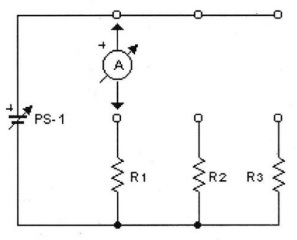
\includegraphics[scale=1.5]{imagenes/9.1}
		\caption{Tercer circuito}
	\end{figure}
	\item Ajuste la salida de la fuente de alimentación de 10 V utilizando el DMM como voltímetro de CC.
	\item Lleve  el DMM al modo de amperimetro y seleccione la escala de 20 mA. Conecte el  como se muestra en la figura 3.
	\item Mida la corriente y registre los valores obtenidos, corriente en:
	\\$R_{1}= 2.56 mA$
	\\$R_{2}= 4.58 mA$
	\item En los pasos 5 a 7 se varió la corriente y se anotaron los valores de tensión en bornes de cada resistor.
	\\ Utilizando los resultados del cuadro 1 de mediciones de la tensión, dibuje un gráfico de la tensión en función de la corriente y denomínelo figura 3 y 4 en las misma graficas para $R_{1}$ y $R_{2}$.
	\\
	\\
	\\
	\\
	\\
	\\
	\begin{figure}[h]
		\centering
		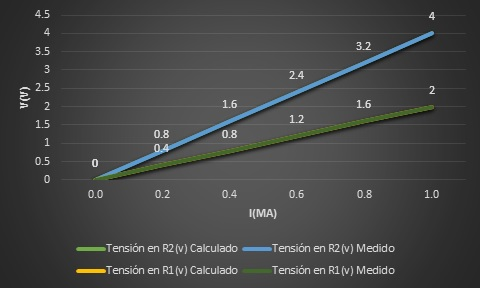
\includegraphics[scale=1]{imagenes/1}
	\end{figure}
	\\
	\\
	Utilizando la ecuación de $V=IR$, calcule la tensión en los bornes de cada resistor para la corriente de 0.5 mA, y marque los puntos en el gráfico con una "X".
	\begin{figure}[h]
		\centering
		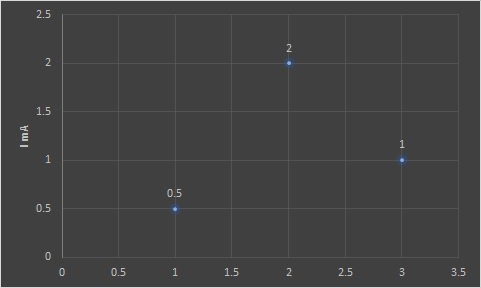
\includegraphics[scale=1]{imagenes/2}
	\end{figure}
	\item En el paso 12  se midió la corriente al variar la resistencia (con  tensión fija de 10 V). Use los resultados del paso 12 y trace una curva de tensión en función de la resistencia.
	\begin{figure}[h]
		\centering
		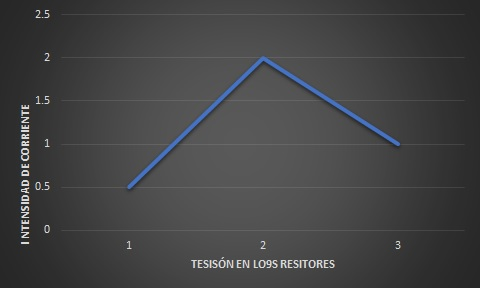
\includegraphics[scale=0.9]{imagenes/3}
	\end{figure}
	\\ Calcule el valor de la resistencia que proporciona un intensidad de 5 mA y una tensión de 10 V, utilizando la ecuación de $R=V/I$ y marcando los puntos en el gráfico con una "X". 
	\\$R_{calculatada}=2k\Omega$ 
	\begin{figure}[h]
		\centering
		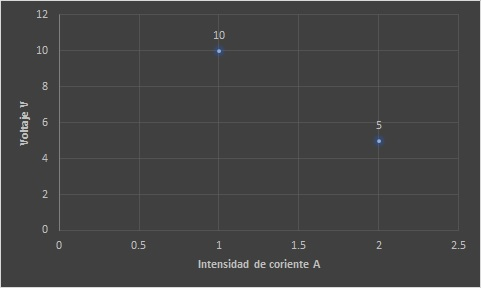
\includegraphics[scale=1]{imagenes/4}
	\end{figure}
	\end{enumerate}
\section{Autoevaluación}
\begin{enumerate}
	\item La tensión en los bornes de un resistor es directamente proporcional al voltaje que circula en la resistencia.
	\item La pendiente de la curva $I=f(V)$ es, 
	\item Al aumentar la resistencia a la tensión constante,
	\item Si pudieran medirse la tensión en los bornes y la corriente en un resistor ¿Cuántas mediciones serían necesarias para determinar su resistencia?
	\item Se midió una tensión de 2,4 V en los bornes de un resistor de $4,7 k \Omega$. La corriente vale 0.51 mA.
\end{enumerate}
\section{Conclusión}
En este laboratorio se llego a aprender como se halla la corriente en una resistencia, puesto que el valor medido es un poco diferente al valor calculado. Todo haciendo uso del multímetro y uso de la ley de Ohmm.